\documentclass[class=article,border=0pt]{standalone}
\pagestyle{empty}

\usepackage{tikz}
\usepackage{tumcolor}

\begin{document}
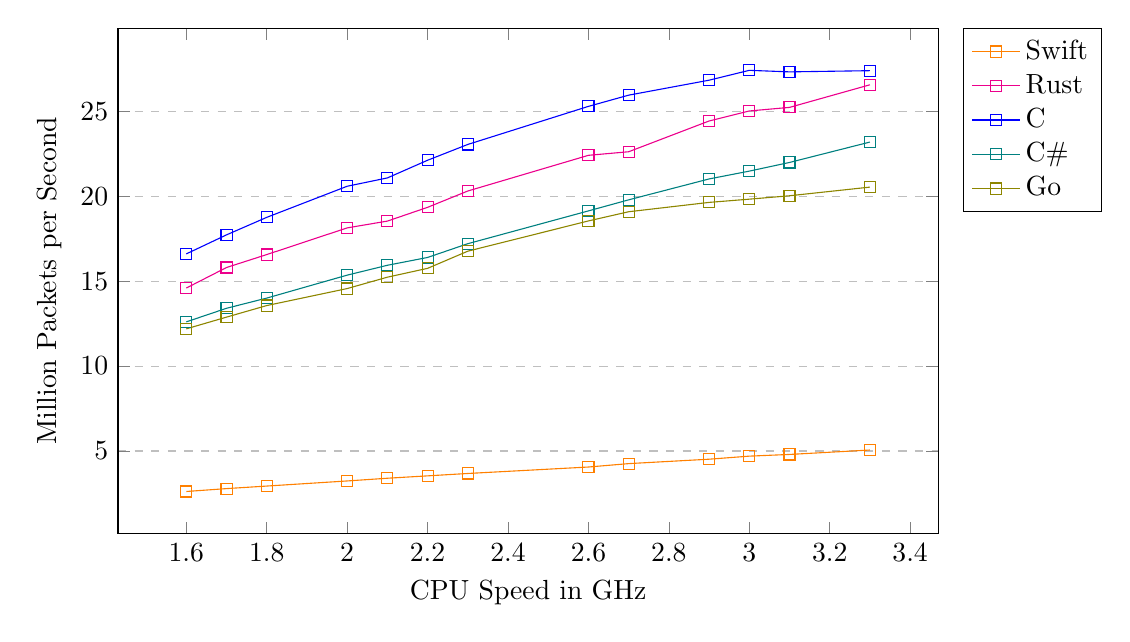
\begin{tikzpicture}
	\begin{axis}[
		width=12cm,
		height=8cm,
		xlabel={CPU Speed in GHz},
		ylabel={Million Packets per Second},
		legend pos=outer north east,
		legend cell align={left},
		ymajorgrids=true,
		grid style=dashed,
	]

		\addplot[
			color=orange,
			mark=square,
			]
			coordinates {
				(1.6, 2.62)(1.7, 2.79)(1.8, 2.94)(2.0, 3.24)(2.1, 3.40)(2.2, 3.54)(2.3, 3.68)(2.6, 4.06)(2.7, 4.26)(2.9, 4.52)(3.0, 4.70)(3.1, 4.80)(3.3, 5.06)
			};

		\addplot[
			color=magenta,
			mark=square,
			]
			coordinates {
				(1.6, 14.59)(1.7, 15.80)(1.8, 16.56)(2.0, 18.13)(2.1, 18.53)(2.2, 19.34)(2.3, 20.30)(2.6, 22.40)(2.7, 22.61)(2.9, 24.42)(3.0, 25.01)(3.1, 25.22)(3.3, 26.55)
			};

		\addplot[
			color=blue,
			mark=square,
			]
			coordinates {
				(1.6, 16.60)(1.7, 17.72)(1.8, 18.75)(2.0, 20.58)(2.1, 21.07)(2.2, 22.11)(2.3, 23.04)(2.6, 25.28)(2.7, 25.94)(2.9, 26.82)(3.0, 27.40)(3.1, 27.31)(3.3, 27.38)
			};

		\addplot[
			color=teal,
			mark=square,
			]
			coordinates {
				(1.6, 12.60)(1.7, 13.40)(1.8, 14.00)(2.0, 15.35)(2.1, 15.93)(2.2, 16.39)(2.3, 17.20)(2.6, 19.13)(2.7, 19.78)(2.9, 21.01)(3.0, 21.47)(3.1, 21.98)(3.3, 23.18)
			};

		\addplot[
			color=olive,
			mark=square,
			]
			coordinates {
				(1.6, 12.19)(1.7, 12.88)(1.8, 13.56)(2.0, 14.56)(2.1, 15.23)(2.2, 15.75)(2.3, 16.76)(2.6, 18.54)(2.7, 19.08)(2.9, 19.63)(3.0, 19.82)(3.1, 20.02)(3.3, 20.53)
			};
		\legend{Swift, Rust, C, C\#, Go}
	\end{axis}
\end{tikzpicture}

\end{document}
